\title{
    \textbf{Domain Analysis\\
    \large Conceptual Documentation}
}
\author{
    Fabio Cosimo Andriulo (s0558214),
    \\Felix Frömel (s0558420),
    \\Lucas Larisch (s0558070)
    \\
    \\ \large \textit{W3-BDA: Big Data Analytics}
    \\ HTW Berlin, University of Applied Sciences
}
\date{July 03, 2021}

%---settings---
\documentclass[11pt]{article} % 11pt or 12pt

\usepackage{lmodern}
\usepackage[utf8]{inputenc}
\usepackage[english]{babel}
\usepackage[T1]{fontenc}
\usepackage{microtype}
\usepackage[backend=biber, urldate=long, dateabbrev=false]{biblatex}
\usepackage[all]{nowidow}
\usepackage{graphicx}
\usepackage{rotating}
\usepackage{setspace}
\usepackage{float}
\usepackage[bottom]{footmisc} % stick footnotes to the bottom (Not explicitly required)
\usepackage[hidelinks]{hyperref}
\usepackage[a4paper, total={210mm,297mm}, left=25mm, right=25mm, top=30mm, bottom=20mm]{geometry}
\usepackage[dvipsnames]{xcolor}
\usepackage{fancyvrb}

\bibliography{literature}
\setstretch{1.3} % 1.3 - 1.5
\setlength{\parskip}{6pt}
\setlength{\footnotesep}{0pt}
\renewcommand{\footnotesize}{\fontsize{9pt}{11pt}\selectfont}

\graphicspath{ {./images/} }

%---content---
\begin{document}
    \pagenumbering{gobble}
    \maketitle
    \pagebreak
    \pagenumbering{Roman}
    \tableofcontents

%---sections---
    \pagebreak
    \setcounter{page}{1}
    \pagenumbering{arabic}

    \section{Introduction:}\label{sec:introduction}
Domain information can change fast due to various reasons such as changes in ownership, the provider as well as of the servers or their locations.
Keeping track of these changes and provide current analyses in the field of related businesses areas require the establishment of processes and strategies for information retrieval, processing, loading, and deployment.
Each of these steps should be realized using state-of-the-art techniques and technologies to enable continuous usage of the product.
Quality measures like code versioning and documentation are fundamental requirements that meet this demand.
This project aims at offering these characteristics and apply them to the field of big data analyses in the topic of domain information retrieved from DNS records.
    \pagebreak
    \section{From Raw Data To Valuable Information}\label{sec:from-raw-data-to-valuable-information}

\subsection{Business Understanding}\label{subsec:businessunderstanding}
The given data includes DNS record information concerning '.de' domains, the country code top-level domains (ccTLD's)~\autocite[cf.][]{DENICeG.2021} allocated to the Federal Republic of Germany.
The comma-separated value file (CSV) with a size of about 500 megabytes contains \textit{.de-related domain names, mail servers used, the domains target IPv4 address, and the timestamp, the information were fetched}.
As CSV files offer straightforward integration into software systems and programs supporting the format~\autocite[cf.][]{Hoffman.2018}, complex file conversion steps (possibly using proprietary software) are not necessary.
Nevertheless, checking the content for correct set delimiters, unnecessary characters, and determination of reasonable data types for subsequent conversion is crucial.
Therefore, we implemented an ETL process to cover these checks and considerations, while ensuring a certain level of flexibility concerning the data sources.

Another important part is the enhancement of the given data by statistics to gain more value out of the data.
As the amount of data and processes to handle them offer various analyses, the following objectives of the project were determined:
\begin{itemize}
    \item Follow the approach ‘everything as code’
    \item Validate existing and collect additional information
    \item Establish an ETL process and data preparation as a requirement for the analyses
    \item Analyses and deployment of the results
\end{itemize}
These objectives as well as the processes explained in the following sections are supposed to provide detailed analysis of DNS record information within the context of big data.


% Beschreibungen und Komentare aus https://www.bigdata-insider.de/was-ist-crisp-dm-a-815478/

\subsection{Data Understanding ...}\label{subsec:dataunderstanding}
After the concrete goals and requirements have been defined in the Business Understanding phase, a close look is taken at the existing basic data.
The existing data is to be examined for processability, content and quality~\autocite[cf.][]{Semmelmann.2020}.
Initial analyses show that the data is available in a comma-separated value structure and is assigned to the context of the Domain Name System (DNS).
Furthermore, the dataset consists of 4 columns and 4860885 rows.
Due to the large amount of data, the use of parallel data processing technologies is inevitable.
To gain an understanding of the data, it is described below:

\begin{center}
    \begin{tabular}{||c c c c||} 
    \hline
    Column & Description & Occurrence & Nullable \\ [0.5ex] 
    \hline\hline
    A & Top-level domains, excluding subdomains & unique & false \\ 
    \hline
    B & MX record from name server & multiple & true \\
    \hline
    C & A-record of the respective domain & multiple & true \\
    \hline
    D & Dolumn D: Timestamp of scraping process & multiple & false
   \end{tabular}
   \end{center}

\begin{itemize}
    \item Erster Überblick über die Daten (Welche Daten, gibt es Probleme)
    \item Probelme insbeosndere in Bezug auf die im vorherigen Kapitel benannten Ziele/Aufgabenstellung/Vorgehensweise
\end{itemize}

\subsection{Data Preparation}\label{subsec:datapreparation}
Data preparation is an essential process beforehand any analysis and thus, should be well documented within the project.
Therefore, Jupyter notebooks containing the associated steps in code blocks were used to provide the processed information.
The code blocks were commented on or being accompanied by explanations to ensure transparency and to match best practices in coding~\autocite[cf.][]{Kosourova.2021}.
The file names are numbered so that the notebooks should be executed consecutively to ensure a clean and smooth delivery of the results.

At first, the required functions are loaded to make them available in the following notebooks.
Afterward, the ETL process is carried out to load the data from the PostgreSQL database, cleaning them (removing special characters and empty lines) and provide the basic data frame for further information processing.
Another enhancement is envisaged by certain checks of the data such as checking the occurrence of 'localhost' entries for mail servers and counts to determine the top ten records (e.g.\ a records) before data are stored in the database.
Furthermore, the existing information is checked for correctness as DNS entries and domains themselves could have changed in the meantime.
This is done by using Pythons dnspython (and various further) package(s) to send requests, fetch the information, and compare them with the original entries if necessary.
To ensure detailed analyses, it is important to collect suitable information which is why we decided to perform the following steps of data retrieval:
\begin{itemize}
    \item Current IP addresses and MX Servers (in comparison to the given data)
    \item HTTP status code per domain and redirects applied to certain domains
    \item Collection of details such as the number of nameservers used per domain and the availability of IPv6 per domain
    \item Company details concerning MX servers and the server of authority (SOA)
    \item Configuration details of the authoritative nameserver (refresh and minimum setting)
\end{itemize}
These steps were performed on extracts of the given dataset as its amount could interfere with performant coding.
As this amount requires corresponding processing steps, parallelization is essential to achieve reasonable runtimes within each code block, which is why we use PySpark, offering native parallelization by using its variant of data frames~\autocite[cf.][]{Weber.2019}.

A key result of this step was the knowledge, that provided data set contains partially outdated information (e.g.\ A- and MX-records of a top-level domain), that some domains are re-directed or that requesting them raised an HTTP errors code.
The methods listed above were focused to encounter these issues.

\subsection{Modeling}\label{subsec:modeling}
Models used in data mining were not implemented within the project in favor of detailed descriptive analyses of the results gained by the steps described before.
The application of reasonable models like pattern recognition (e.g. Clustering methods) may require further data that could be realized in a follow-up project.
However, this is a challenging task concerning information retrieval, data storage, and loading which requires further enhancements and awareness of performance issues.

\subsection{Evaluation}\label{subsec:evaluation}
As models were not used within this project, an evaluation of such was not done.
Re-evaluation of created models would be a continuous step in the project to keep track of changing requirements (analyses) and of the frequent changes of the data justified on the given context.

\subsection{Deployment}\label{subsec:deployment}
For details concerning deployment, see section~\ref{sec:project-realization}.
    \pagebreak
    \section{Project Realization}\label{sec:project-realization}

\subsection{Dockerized Microservices as Infrastructure}\label{subsec:dockerized-microservices-as-infrastructure}

Aiming for short feedback-loops, and the prevention of shipping anything but code, the domain analysis project has been realized following the principles of \textit{Infrastructure as Code}, a procedure that is at DevOps' core.~\autocite[cf.][p. 13]{Riti.2018}
More specifically, the project consists of five dockerized services that are
managed using \textit{Docker Compose} and communicating with each other through a Docker network.
Unless stated otherwise, the containers are only communicating through this network, i.e.\ their port is not mapped.
In the following, these services as well as how they are interacting will be described briefly.
All Dockerfiles as well as the docker-compose file can be found in~\ref{subsec:docker-compose} -~\ref{subsec:dockerfile-(dig-microservice)}.

\subsubsection{PySpark Jupyter Lab}\label{subsubsec:pyspark-jupyter-lab}

In order to process the data described in the previous chapter efficiently, a Jupyter Lab running PySpark, customized regarding the requirements of the analyses to be made, is used.
The container is accessible from the host machine on port \texttt{8888} using the token \texttt{token4711} and, due to mounting both the notebooks containing the code to be executed,
and the data to be analyzed, it can be used for working without the risk of losing information on removing the container.
Eventually, the processed data is stored in the Postgres database described in ~\ref{subsubsec:postgres-database}.
%

\subsubsection{Postgres Database}\label{subsubsec:postgres-database}

For storing the enhanced data, a Postgres database is used which is initialized with all tables to be used for the domain analysis, functions for getting the data to be displayed as charts/KPIs (cf.~\ref{subsubsec:dashboard})
and notifier functions/triggers for asynchronous communication to be described in~\ref{subsec:event-driven-architecture}.

\subsubsection{Statistics Service}\label{subsubsec:statistics-service}

The Statistics Service collects data to be displayed from the Postgres database (cf.~\ref{subsubsec:postgres-database}) and asynchronously sends it the connected dashboards (cf.~\ref{subsubsec:dashboard}) using Web Sockets.~\autocite[cf.][]{MDNWebDocs.2021}

\subsubsection{Dashboard}\label{subsubsec:dashboard}

The dashboard container runs an Angular application that is accessible on port \texttt{8321} and visualizes the data received from the Statistics Service dynamically.
Its layout is card- and tab-based in order to prominently display the data to be presented and dividing it into logically coherent sections.
Information will either be displayed as a KPI or as a chart component.
Furthermore, it contains a mocked terminal for performing requests to the Dig Service presented in ~\ref{subsubsec:dig-microservice}.

\subsubsection{Dig Microservice}\label{subsubsec:dig-microservice}

Even though its usage within the scope of this project's data analysis part was discarded as the required functionality was solved in another way, the Dig Microservice allows performing \texttt{dig}-requests through HTTP due to running in a container based on Linux Debian.

\subsection{Benefits of Using Node.js}\label{subsec:choosing-a-node-based-environment}

Both the dig microservice, and the statistics service are Node.js applications written in TypeScript.
In this project's context, this was a deliberate decision considering several aspects to be described in the following.

First, it is of the utmost importance to understand the concept of microservices, i.e.\ only solving one, or a limited number of tasks.
If application logic was to be supplemented, another microservice would be created, resulting in a distributed system instead of extending the scope of one service.~\autocite[cf.][p. 23]{Farcic.2016}
Since, in this context, the tasks of both services in themselves are not related to data science, it is not necessary to use a programming language commonly related to this topic such as Python or R.~\autocite[cf.][]{Gossett.2021}

Furthermore, it is possible to implement custom packages shared by multiple containers.
Within the scope of this project, \texttt{domain-analysis-types}, an NPM package used by both the dashboard, and the statistics service is built which centrally defines names of events (cf.~\ref{subsec:event-driven-architecture}).
Subsequently, complexity is minimized as a predefined list of events is used on both ends and if an event name is changed, it is changed for both the client and the server.

Last but not least, for dockerizing the dashboard project, a Node.js image (\texttt{node:16-alpine}) is used in the build step.
Considering base images are only downloaded once and referenced by each container, using the same base image for multiple minimizes the disk space to be used, and the time for initially building all images.~\autocite[cf.][pp. 8-9]{Arundel.2019}

\subsection{Event-driven Architecture}\label{subsec:event-driven-architecture}

In order to improve the user experience (UX), the dashboard is loaded asynchronously.~\autocite[cf.][]{Shah.2021}
Therefore, using Socket.io, it subscribes to events emitted from the statistics service and updates the respective values dynamically.
On connecting, the client (only this instance) receives the data for all events from the statistics service.

The server, on the other hand, subscribes to notifications from the database.
In order to avoid sending an unnecessary amount of data, the payload emitted by the database is always \texttt{NULL}, i.e.\ subscribers are only informed about changes but not about what has changed.
After not receiving any new notification from the database for 2 seconds, the statistics service emits the updated data to all clients, i.e.\ it requests the respective data from the database using a predefined database function and emits it eventually.

    \pagebreak
    \section{Closing Remarks}\label{sec:closing-remarks}

\subsection{License (CC-BY-NC-4.0)}\label{subsec:license}

\subsection{Project Repository}\label{subsec:project-repository}

\subsubsection*{Start and shut down this project ...}


%---sources---
    \pagebreak
    \pagenumbering{Roman}
    \setcounter{page}{2}

    \addcontentsline{toc}{section}{References}
    \printbibliography

%---declaration of authorship, permission for sharing & appendix ---
    \pagebreak
    \section*{Declaration of Authorship}
\addcontentsline{toc}{section}{Declaration of Authorship}

Hereby, we declare the presented conceptional documentation to have been composed independently on our own and without any other resources than the ones indicated.
All thoughts taken directly or indirectly from external sources are properly denoted as such.

\vspace{15mm}

{\setlength{\parindent}{0cm}
    Berlin, 04.07.2021

    Fabio Cosimo Andriulo,
    Felix Frömel,
    Lucas Larisch
}

    \pagebreak
    \section*{Permission for Sharing This Conceptional Documentation}
\addcontentsline{toc}{section}{Permission for Sharing This Conceptional Documentation}

Hereby, we grant permission for sharing both this essay and its related presentation for educational purposes.

\vspace{15mm}

{\setlength{\parindent}{0cm}
Berlin, 03.07.2021

Fabio Cosimo Andriulo,
    Felix Frömel,
    Lucas Larisch
}

    \pagebreak
    \appendix
\section{Appendices}\label{sec:appendices}

\subsection{Dashboard Sections (KPIs and Charts)}\label{subsec:dashboard-sections-(kpis-and-charts)}

{\setlength{\parindent}{0cm}\textbf{\textit{1) Descriptive Information}}}
\begin{itemize}
    \item \textbf{KPI 1:} Total number of parsed domains
    \item \textbf{KPI 2:} Percentage of domains with "localhost" as MX-record
    \item \textbf{Chart 1:} Most common MX-records (Top 10)
    \item \textbf{Chart 2:} Most common A-records (Top 10)
    \item \textbf{Chart 3:} Grouped number of MX-records per domain
    \item \textbf{Chart 4:} Grouped number of A-records per domain
\end{itemize}

{\setlength{\parindent}{0cm}\textbf{\textit{2) Updated Records}}}
\begin{itemize}
    \item \textbf{KPI 1:} Percentage of domains with "localhost" as MX-record (updated)
    \item \textbf{KPI 2:} Percentage of changed A-records (excluding request errors)
    \item \textbf{KPI 3:} Percentage of changed MX-records (excluding request errors)
    \item \textbf{Chart 1:} Most common (updated) MX-records (Top 10)
    \item \textbf{Chart 2:} Most common (updated) A-records (Top 10)
    \item \textbf{Chart 3:} Grouped number of (checked) MX-records per domain
    \item \textbf{Chart 4:} Grouped number of (checked) A-records per domain
\end{itemize}

{\setlength{\parindent}{0cm}\textbf{\textit{3) Accessibility}}}
\begin{itemize}
    \item \textbf{KPI 1:} Percentage of redirections (excluding null values)
    \item \textbf{KPI 2:} Percentage of redirections with status code 200 (excluding null values)
    \item \textbf{Chart 1:} The domains' status codes
    \item \textbf{Chart 2:} Domains redirected to (Top 10)
\end{itemize}

{\setlength{\parindent}{0cm}\textbf{\textit{4) Mail Servers}}}
\begin{itemize}
    \item \textbf{KPI 1:} Percentage of MX-records from e-mail providers head-quartered outside Germany
    \item \textbf{Chart 1:} Most common e-mail providers (Top 10)
    \item \textbf{Chart 2:} Number of MX-records grouped by provider cities (Top 10)
    \item \textbf{Chart 3:} Number of MX-records grouped by provider countries (Top 10)
\end{itemize}

{\setlength{\parindent}{0cm}\textbf{\textit{5) IPv6, SOA Details and Companies}}}
\begin{itemize}
    \item \textbf{KPI 1:} Percentage of domains supporting IPv6 (excluding request errors)
    \item \textbf{KPI 2:} Average SOA "Minimum" value in seconds
    \item \textbf{KPI 3:} Average SOA "Refresh" value in seconds
    \item \textbf{KPI 4:} Percentage of nameservers from providers head-quartered outside Germany
    \item \textbf{Chart 1:} Grouped number of nameservers per domain (excluding request errors)
    \item \textbf{Chart 2:} Most common nameserver providers (Top 10)
    \item \textbf{Chart 3:} Number of nameservers grouped by provider cities (Top 10)
    \item \textbf{Chart 4:} Number of nameservers grouped by provider countries (Top 10)
\end{itemize}
\label{dashboardtabsannex}
\pagebreak
\subsection{Project Architecture}\label{subsec:project-architecture}

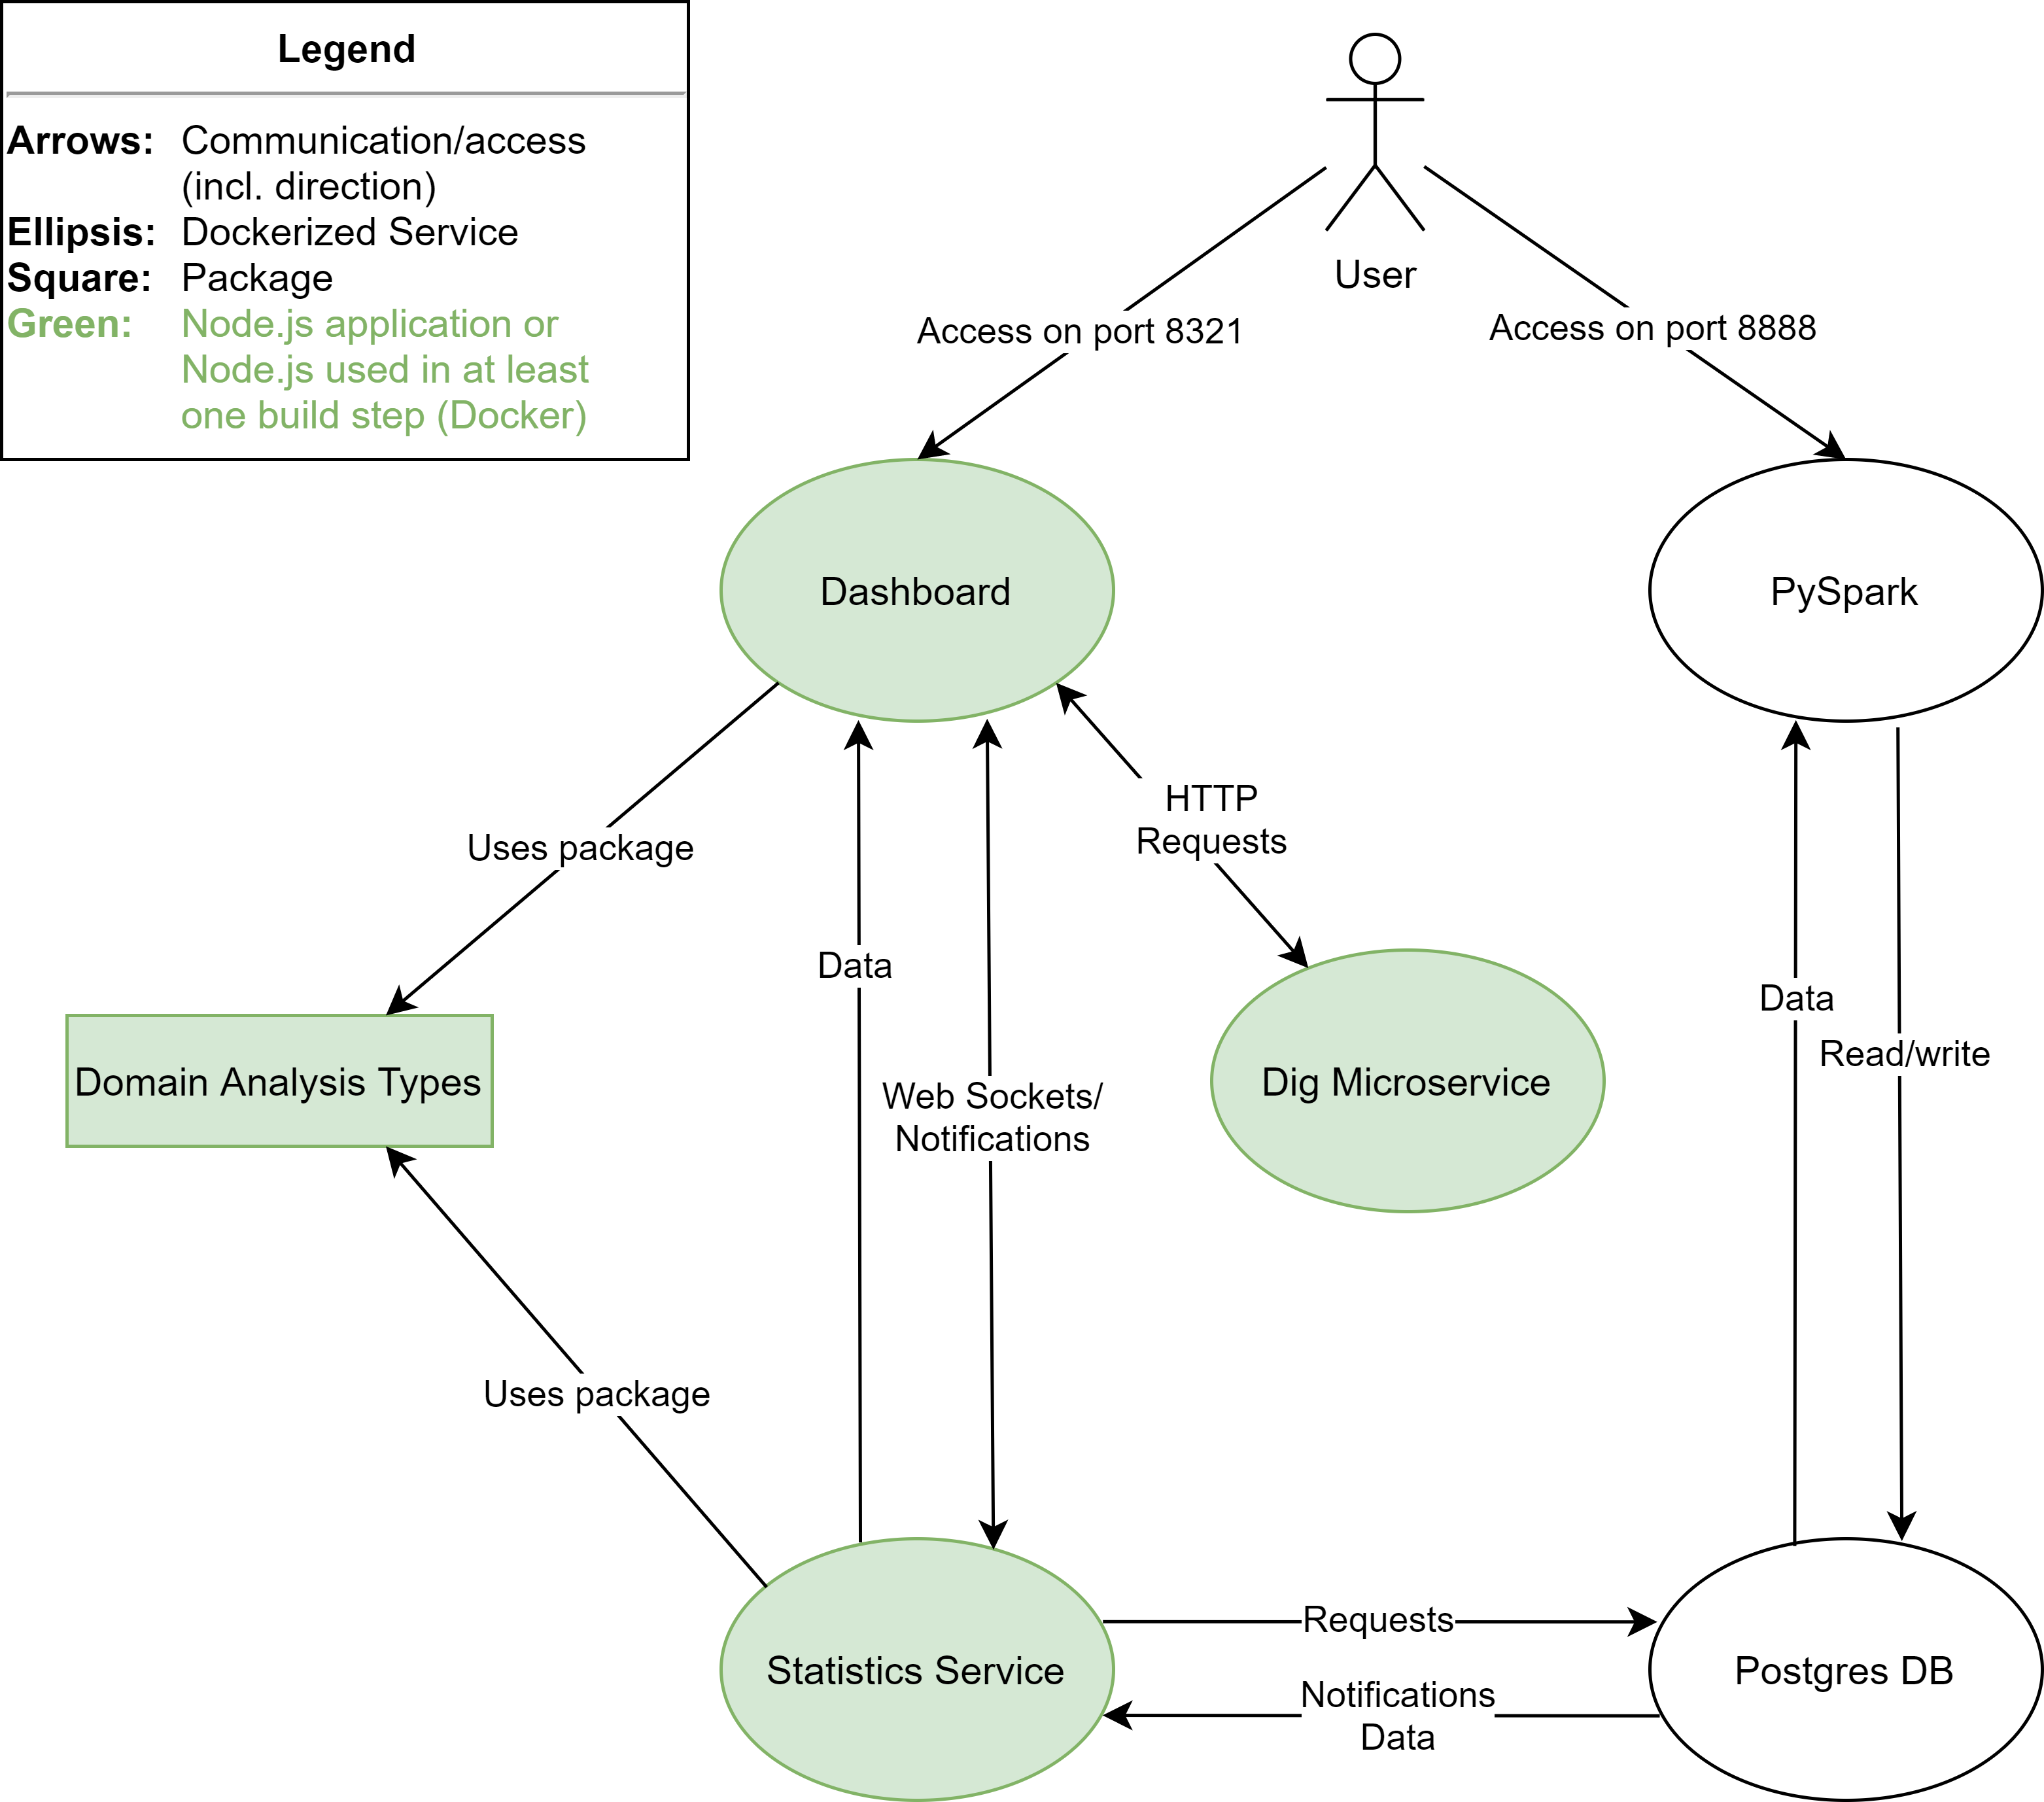
\includegraphics[width=1\textwidth]{../project-architecture}

\pagebreak
\subsection{Docker Compose}\label{subsec:docker-compose}

\RecustomVerbatimCommand{\VerbatimInput}{VerbatimInput}
{fontsize=\footnotesize,
    frame=single,
    framesep=2em,
    rulecolor=\color{Blue},
    label=\fbox{\color{Blue}docker-compose.yml},
    labelposition=bottomline
}

\VerbatimInput{../src/services/docker-compose.yml}

\subsection{Dockerfile (PySpark)}\label{subsec:dockerfile-(pyspark)}

\RecustomVerbatimCommand{\VerbatimInput}{VerbatimInput}
{fontsize=\footnotesize,
    frame=single,
    framesep=2em,
    rulecolor=\color{Blue},
    label=\fbox{\color{Blue}Dockerfile (PySpark)},
    labelposition=bottomline
}

\VerbatimInput{../src/services/pyspark/Dockerfile}

\subsection{Dockerfile (Postgres)}\label{subsec:dockerfile-(postgres)}

\RecustomVerbatimCommand{\VerbatimInput}{VerbatimInput}
{fontsize=\footnotesize,
    frame=single,
    framesep=2em,
    rulecolor=\color{Blue},
    label=\fbox{\color{Blue}Dockerfile (Postgres)},
    labelposition=bottomline
}

\VerbatimInput{../src/services/postgres-db/Dockerfile}

\subsection{Dockerfile (Statistics Service)}\label{subsec:dockerfile-(statistics-service)}

\RecustomVerbatimCommand{\VerbatimInput}{VerbatimInput}
{fontsize=\footnotesize,
    frame=single,
    framesep=2em,
    rulecolor=\color{Blue},
    label=\fbox{\color{Blue}Dockerfile (Statistics Service)},
    labelposition=bottomline
}

\VerbatimInput{../src/services/statistics-service/Dockerfile}

\subsection{Dockerfile (Dashboard)}\label{subsec:dockerfile-(dashboard)}

\RecustomVerbatimCommand{\VerbatimInput}{VerbatimInput}
{fontsize=\footnotesize,
    frame=single,
    framesep=2em,
    rulecolor=\color{Blue},
    label=\fbox{\color{Blue}Dockerfile (Dashboard)},
    labelposition=bottomline
}

\VerbatimInput{../src/services/dashboard/Dockerfile}

\subsection{Dockerfile (Dig Microservice)}\label{subsec:dockerfile-(dig-microservice)}

\RecustomVerbatimCommand{\VerbatimInput}{VerbatimInput}
{fontsize=\footnotesize,
    frame=single,
    framesep=2em,
    rulecolor=\color{Blue},
    label=\fbox{\color{Blue}Dockerfile (Dig Microservice)},
    labelposition=bottomline
}

\VerbatimInput{../src/services/dig-microservice/Dockerfile}


\end{document}
